\chapter{FOBOS Hardware Configuration} \label{chap:hardware-config}
\section{Oscilloscope Interface}
Ocsilloscope is connected to the PC via IP netwok. IP configuration must be done on the oscilloscope for the PC to be able to collect traces. The oscillopscope used in tests is Agilent DSO6054A. To configure IP on this oscilloscope, please refer to vendor's documentation.

\section{Crypto Algorithm Wrapper}
The Victim Board runs the cipher that need to be attcked (user provided). A victim wrapper is included to facilitate communication between FOBOS Control Board and Victim Board. After the wrapper gets the data from the Control Board, it sends it to the victim cipher. After the victim cipher finishes, result is transfered back to the Control Board.
Here we list signals used to interface between the victim wrapper and victim cipher:

\begin{enumerate}
\item clock : clock signal from the Control Board used to drive Victim Board.
\item data\_to\_crypto : A block of data to be processed by the victim cipher.
\item key\_to\_crypot : The key used by victim cipher.
\item data\_out : result of victim cipher.
\item start : A handshake signal indcating the data\_to\_crypto and key\_to\_crypto are valid and instructs victim cipher to start processing.
\item done : A handshake signal generated by victim cipher to indcate that processing finished and data\_out is valid result.
\end{enumerate}

\section{Control Board Programming}

There are two generic parameters that need to be configured depending on the Control board used.
The \texttt{Interface\_Width} generic is the width of the bus used to communicate between the Control and Victim boards (in each direction). The \texttt{board} generic is used to indicate the type of control board used. These values are set in the \texttt{\$fobos/sources/common/fobos-package.vhd} file. For valuse, refer to Table ~ \ref{tab:interface-width}.

\begin{table}[H]
  \begin{center}
    \caption{\label{tab:interface-width}Interface\_Width Parameter}
    \begin{tabular}{|p{4cm}|p{2cm}|p{2cm}|}
    	\hline
       Control Board & Interface\_Width & Board\\ \hline
       Nexys2 & 16 & 1 \\ \hline
       Nexys3 & 4 & 2 \\ \hline
  \end{tabular}
  \end{center}
\end{table} 
After the generics have been edited, the FPGA can now be programmed as follows:
\begin{enumerate}
  \item Create a new project using Xilinx ISE. In the New Project wizard set the Project Settings per the Control Board used. Make sure to select the values for Family, Device, Package and Speed (See Fig~\ref{fig:ctrl-design-properties} for an example).
  		\begin{figure}[H]
		\begin{center}
		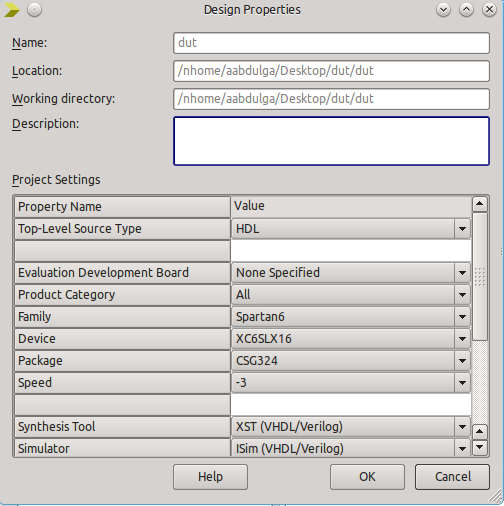
\includegraphics[scale=0.6]{figures/ctrl-design-properties}
		\caption{\label{fig:ctrl-design-properties}FOBOS Controller Desgin Properties}
		\end{center}
		\vspace{-1ex}
		\end{figure}
  \item From the Project menu, select Add Source... and add all files from \texttt{\$fobos/sources/common}.
  \item Repeat the previous process to add all vhdl files from \texttt{\$fobos/sources/vhdl/control}. Also, add the appropriate UCF file depending on the Control Board used (See Fig~\ref{fig:ctrl-add-sources}) .
		\begin{figure}[H]
		\begin{center}
		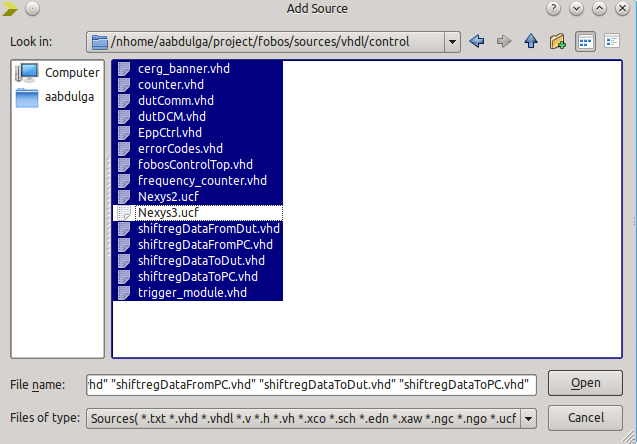
\includegraphics[scale=0.6]{figures/ctrl-add-sources}
		\caption{\label{fig:ctrl-add-sources}Adding Source Files to FOBOS Controller}
		\end{center} 
		\vspace{-1ex}
		\end{figure}
  \item Set the \texttt{fobosControlTopLevel} module as the top-level module for this project (See Fig~\ref{fig:ctrl-set-top-level}).
		\begin{figure}[H]
		\begin{center}
		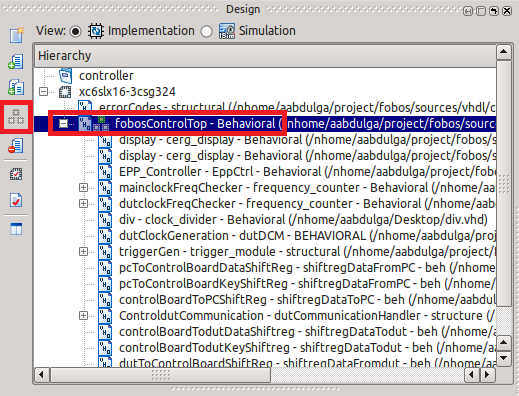
\includegraphics[scale=0.6]{figures/ctrl-set-top-level}
		\caption{\label{fig:ctrl-set-top-level}Setting Top-level Module}
		\end{center} 
		\vspace{-1ex}
		\end{figure}
  \item Generate the programming bit file for the control board by clicking "Generate Programming File" in the Processes window.
  \item Program the control board using Xilinx Impact. In the Processes window, click Configure Target Device (See Fig~\ref{fig:ctrl-run-impact}).
		\begin{figure}[H]
		\begin{center}
		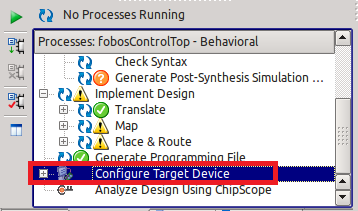
\includegraphics[scale=0.6]{figures/ctrl-run-impact}
		\caption{\label{fig:ctrl-run-impact}}
		\end{center}
		\vspace{-1ex}
		\end{figure}
  \item In the Impact window, click "Boundary Scan" then form the File menu, click "Initialize Chain" and assign the bit file to the FPGA. Now you may right-click the FPGA and click "Program".
		\begin{figure}[H]
		\begin{center}
		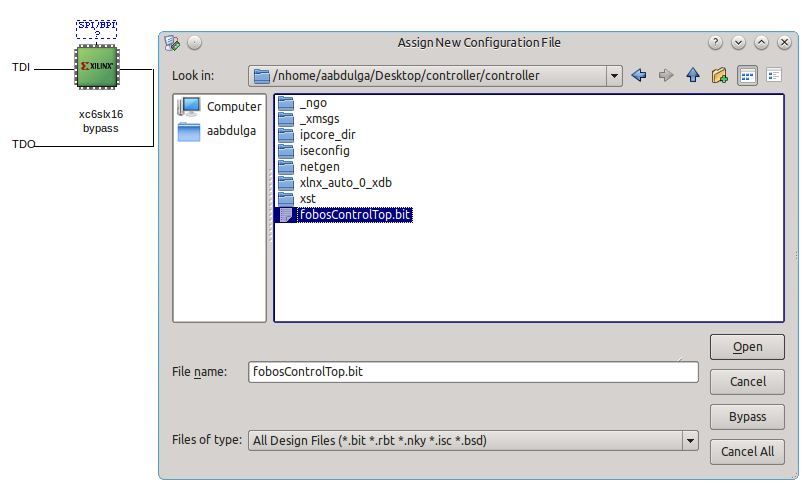
\includegraphics[scale=0.6]{figures/ctrl-program}
		\caption{\label{fig:ctrl-program}Progrmamming Control Board}
		\end{center}
		\vspace{-1ex}
		\end{figure}
  \end{enumerate}

\section{DUT Board Programming}
\begin{enumerate}
  \item Create a new project using Xilinx ISE. In the New Project wizard set the Project Settings per the DUT Board used. Make sure to select the values for Family, Device, Package and Speed (See Fig~\ref{fig:dut-design-properties} for an example).
		\begin{figure}[H]
		\begin{center}
		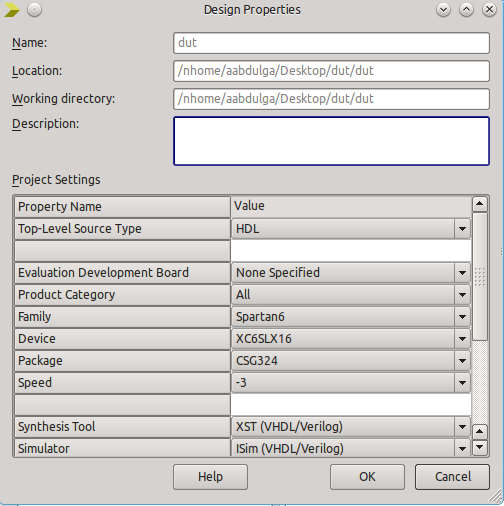
\includegraphics[scale=0.6]{figures/dut-design-properties}
		\caption{\label{fig:dut-design-properties}DUT Design Properties}
		\end{center}
		\vspace{-1ex}
		\end{figure}
  \item From the Project menu select Add Source... and add all files from \texttt{\$fobos/sources/common}.
  \item Repeat the previous process to add all vhdl files from \texttt{\$fobos/sources/vhdl/DUT} and make sure to add the appropriate UCF file depending on the DUT board used (See Fig~\ref{fig:dut-add-sources}).
  	\item Add the victim cipher vhdl files to the project (user provided).
		\begin{figure}[H]
		\begin{center}
		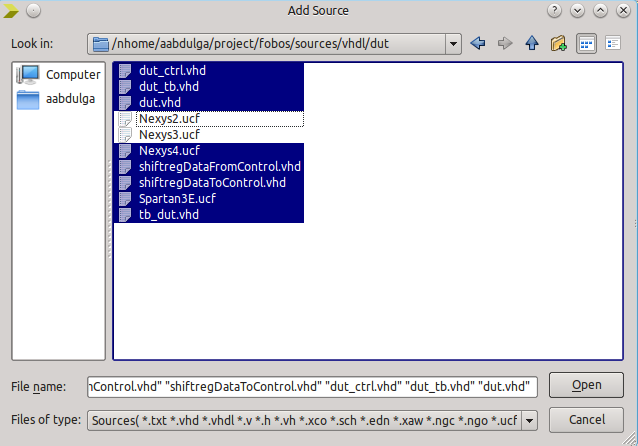
\includegraphics[scale=0.6]{figures/dut-add-sources}
		\caption{\label{fig:dut-add-sources}DUT Add Sources}
		\end{center}
		\vspace{-1ex}
		\end{figure}
  \item Make sure to not use block RAMs in the implementation. .
     \begin{enumerate}
	\item Make sure to select the "Implementation" view.
        \item Right-click the Synthesize-XST process.
	\item In the Preocess Properties window, select HDL Options and select "Distributed" for the RAM Style property (See Fig~\ref{fig:dut-ram-style}).
	\item Click OK.
		\begin{figure}[H]
		\begin{center}
		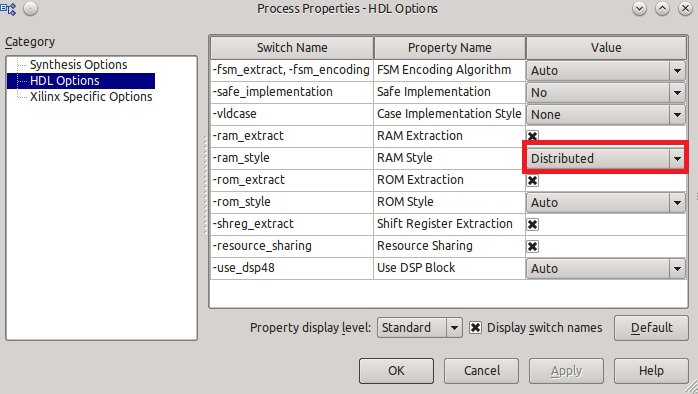
\includegraphics[scale=0.6]{figures/dut-ram-style}
		\caption{\label{fig:dut-ram-style}DUT RAM Style}
		\end{center}
		\vspace{-3ex}
		\end{figure}
     \end{enumerate}
  \item Set the \texttt{dutTopLevel} as the top-level module in this project.
		\begin{figure}[H]
		\begin{center}
		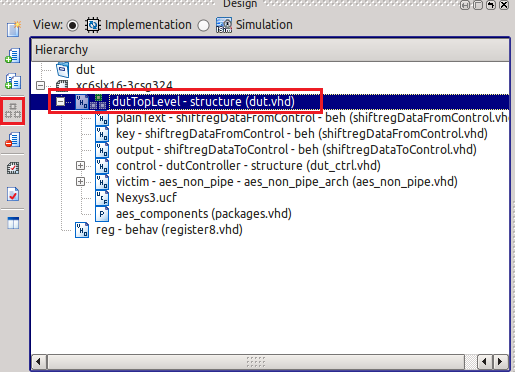
\includegraphics[scale=0.6]{figures/dut-set-top-level}
		\caption{\label{fig:dut-set-top-level}Set DUT Top-level}
		\end{center}
		\vspace{-3ex}
		\end{figure}
  \item Generate the programming bit file for the DUT by clicking "Generate Programming File" in the Processes window.
  \item Program the DUT using Xilinx Impact. In the Processes window, click Configure Target Device (See Fig~\ref{fig:dut-run-impact}).
		\begin{figure}[H]
		\begin{center}
		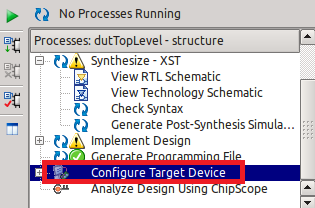
\includegraphics[scale=0.6]{figures/dut-run-impact}
		\caption{\label{fig:dut-run-impact}}
		\end{center}
		\vspace{-3ex}
		\end{figure}
  \item In the Impact window, click "Boundary Scan" then form the File menu, click "Initialize Chain" and assign the bit file to the FPGA. Now you may right-click the FPGA and click "Program".
		\begin{figure}[H]
		\begin{center}
		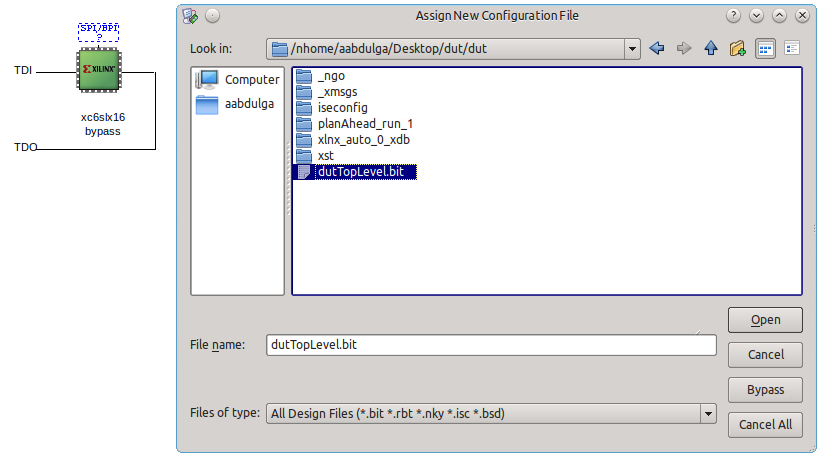
\includegraphics[scale=0.6]{figures/dut-program}
		\caption{\label{fig:dut-program}Progrmamming DUT}
		\end{center}
		\vspace{-3ex}
		\end{figure}
  \end{enumerate}


\section{FOBOS Oscilloscope Configuration}
Oscilloscope need to be conncted to the network and have an IP address and port number. To configure the oscilloscope, refer to vendors's documentation.

\section{Connecting Hardware}

To connect FOBOS hardware, follow these steps:
  \begin{enumerate}
  \item Connect control board to power and ground.
  \item Connect control board tirgger output the oscilloscope channel.
  \item Connect the control board to the DUT.
  \item Connect the control board to the PC running the FOBOS software using USB.
  \item Connect clock generator to control board. Set the clock generator to desired clock.
  \item Connect the current probe to the oscilloscope.
  \item Connect the current probe to the DUT's ground.
  \item Connect DUT to power making sure that the current probe is measuring the current.
  \item Connect DUT to power supply ground.
  \end{enumerate}
  
The following subsections ilustrate how to connect different FPGA boards as control and victim boards.

\subsection{Nexys3 Control Board - Nexys4 DUT}
Illustrated figure 
\subsection{Nexys3 Control Board - Nexys3 DUT}
Illustrated figure
\subsection{Nexys2 Control Board - Spartan3E DUT}
Illustrated figure